\let\negmedspace\undefined
\let\negthickspace\undefined
\documentclass[journal]{IEEEtran}
\usepackage[a5paper, margin=10mm, onecolumn]{geometry}
%\usepackage{lmodern} % Ensure lmodern is loaded for pdflatex
\usepackage{tfrupee} % Include tfrupee package

\setlength{\headheight}{1cm} % Set the height of the header box
\setlength{\headsep}{0mm}     % Set the distance between the header box and the top of the text

\usepackage{cite}
\usepackage{amsmath,amssymb,amsfonts,amsthm}
\usepackage{algorithmic}
\usepackage{graphicx}
\usepackage{textcomp}
\usepackage{xcolor}
\usepackage{txfonts}
\usepackage{listings}
\usepackage{enumitem}
\usepackage{mathtools}
\usepackage{gensymb}
\usepackage{comment}
\usepackage[breaklinks=true]{hyperref}
\usepackage{tkz-euclide} 
\usepackage{listings}
% \usepackage{gvv}  
\usepackage{float}
\def\inputGnumericTable{}                                 
\usepackage[latin1]{inputenc}                                
\usepackage{color}                                        
\usepackage{listings}
\usepackage{array}                                            
\usepackage{longtable}                                       
\usepackage{calc}                                             
\usepackage{multirow}                                         
\usepackage{hhline}                                           
\usepackage{ifthen}                                           
\usepackage{lscape}
\usepackage{multicol}
\begin{document}

\bibliographystyle{IEEEtran}
\vspace{3cm}

\title{Traffic light Controller} 
\author{
EE25BTECH11012-Beeram Madhuri}
% \maketitle
% \newpage
% \bigskip
{\let\newpage\relax\maketitle}

\renewcommand{\thefigure}{\theenumi}
\renewcommand{\thetable}{\theenumi}
\setlength{\intextsep}{10pt} % Space between text and floats


\numberwithin{equation}{enumi}
\numberwithin{figure}{enumi}
\renewcommand{\thetable}{\theenumi}
\textbf{Objective:}\\
To design and implement Traffic light Controller (at a 3 road junction) and to verify its operation using an Arduino-generated clock signal.\\

\textbf{Components used:}
\begin{enumerate}
    \item 2 D Flip-flops(1 74LS74 IC)
    \item AND gate IC
    \item NOR gate IC
    \item 6 LEDs(3 red and 3 green)
    \item Breadboard, Resistors
    \item Voltage and clock sources
\end{enumerate}

\textbf{State Transition table for a 3 road junction Traffic light controller:}\\
For a 3 road junction when one of the road has green signal other 2 should have a red signal ($G_1$ $\rightarrow$ $G_2$ $\rightarrow$ $G_3$)\\
\begin{table}[H]
\centering
\caption{TABLE 1: State Transition table:}
\begin{tabular}{|l|l|c|c|c|}
\hline
\textbf{Present State} & \textbf{} & \textbf{} & \textbf{Next state} \\
\hline
\textbf{$Q_1 Q_0$} & \textbf{$D_1$} & \textbf{$D_0$} & \textbf{$ Q_1 Q_0$} \\
\hline
0 0 & 0 & 1 &  0 1 \\
\hline
0 1& 1 & 0 & 1 0 \\
\hline
1 0& 0 & 0 & 0 0 \\
\hline
1 1& 0 & 0 & 0 0 \\
\hline
\end{tabular}
\label{tab:rc_results}
\end{table}
Hence,\\
$$ D_1 = \overline{Q_1} Q_0 $$
$$ D_0 = \overline{Q_1}.\overline{Q_0} $$

Determining Equations for $G_1, G_2, G_3, R_1, R_2, R_3$:\\

$R_i=\overline{G_i}$ for i=1,2,3.
\begin{table}[H]
\centering
\caption{}
\begin{tabular}{|l|l|c|c|c|}
\hline
\textbf{State: $Q_1 Q_0$} & \textbf{$G_1$} & \textbf{$G_2$} & \textbf{$G_3$} \\
\hline
0 0 & 1 & 0 & 0\\
\hline
0 1& 0& 1 & 0 \\
\hline
1 0& 0 & 0 & 1 \\
\hline
\end{tabular}
\label{tab:rc_results}
\end{table}
$\therefore$ 
\begin{align*}
    G_1=\overline{Q_1}.\overline{Q_0}\\
G_2=\overline{Q_1}Q_0 \\
G_3=\overline{Q_0}Q_1\\
(or)\\
(G_2=Q_0\\
G_3=Q_1)\\
\end{align*}
\text{(as state 11 is used as don't cares for minimization)}


\textbf{Circuit Diagram:}
\begin{figure}[H]
\centering
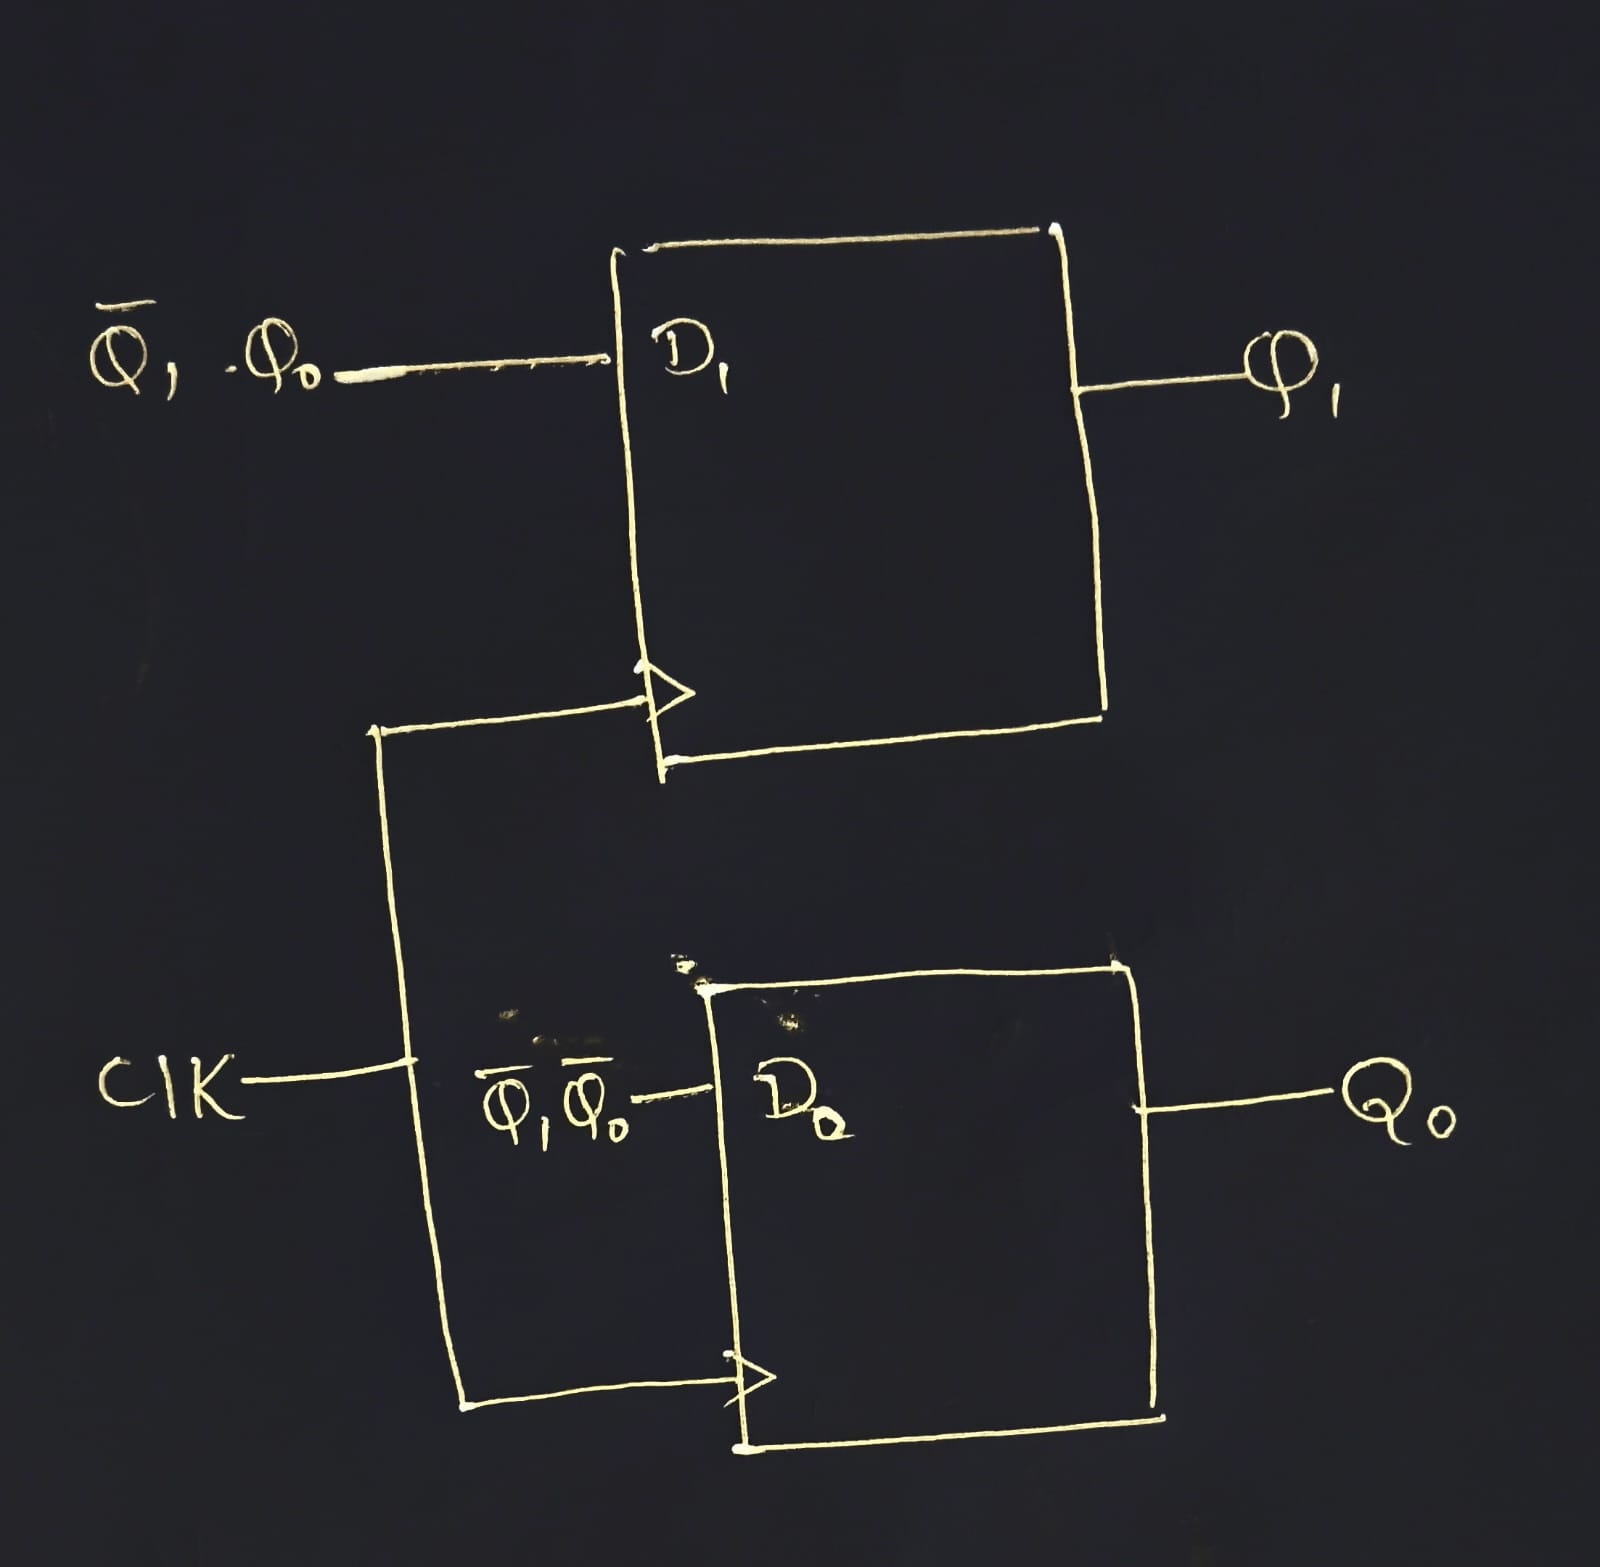
\includegraphics[width=0.4\columnwidth]{Figures/Circuit diagram.jpeg}
\caption{Circuit Diagram}
\label{fig:placeholder}
\end{figure}

\textbf{Breadboard Connections:}
\begin{figure}[H]
\centering
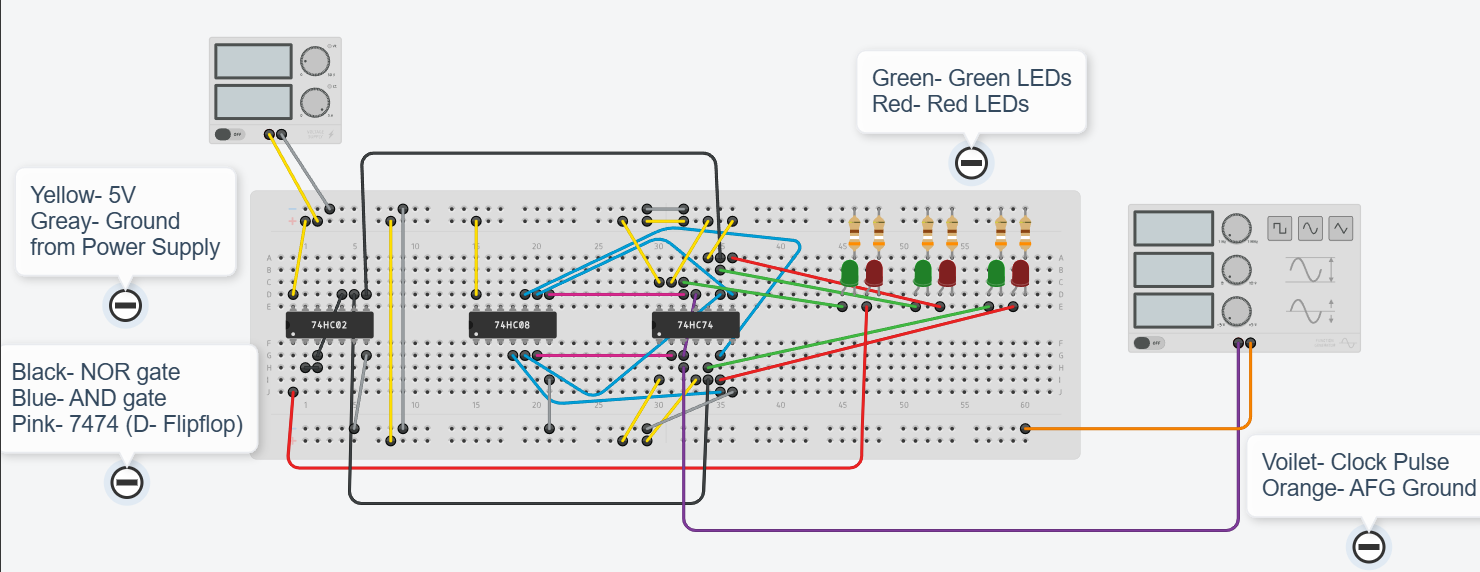
\includegraphics[width=1\columnwidth]{Figures/Circuit view.png}
\caption{Breadboard Connections}
\label{fig:placeholder}
\end{figure}

\textbf{Schematic view of Breadboard Connections:}
\begin{figure}[H]
\centering
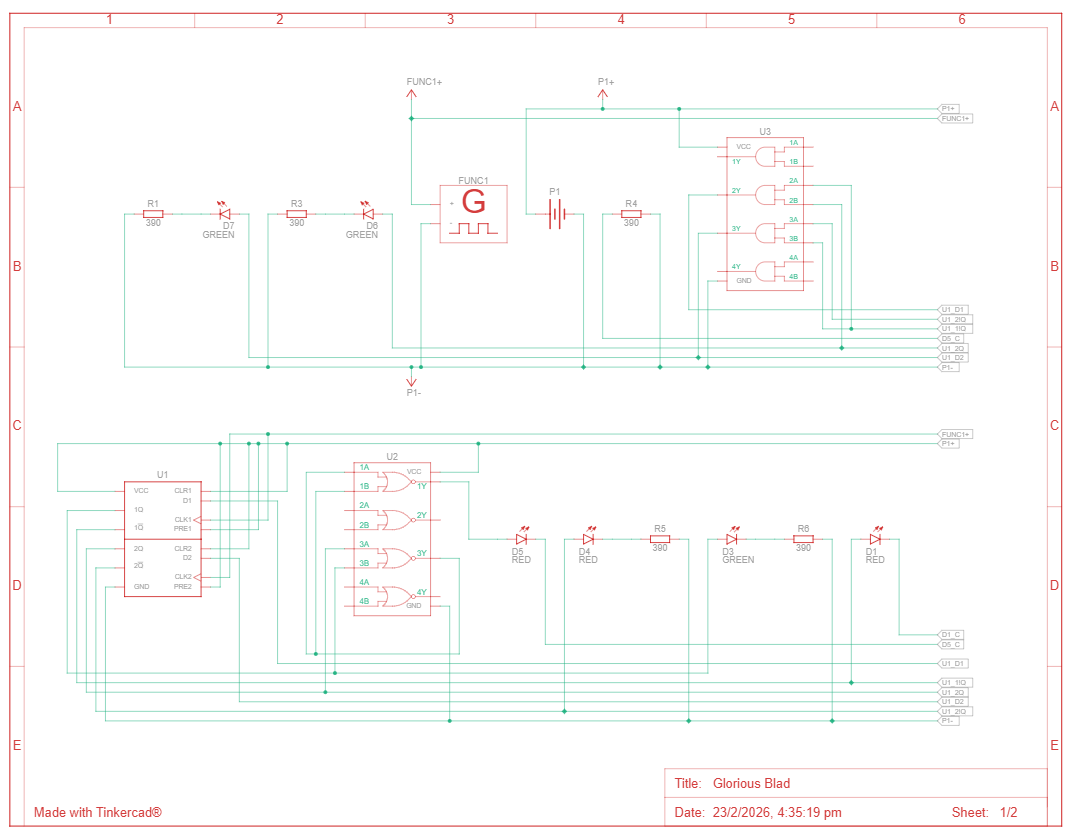
\includegraphics[width=1\columnwidth]{Figures/Schematic view.png}
\caption{Breadboard Connections}
\label{fig:placeholder}
\end{figure}

\textbf{Observation and Troubleshooting:}\\

$\rightarrow$ Problem 1: Faulty Bread Issue\\

\textbf{Observation:}\\
During testing, inconsistent output behavior was observed even after verifying the IC connections and supply voltage.\\

\textbf{Issue Identified:}\\
The solderless breadboard had internal contact strip damage or loose internal connections, causing unreliable signal transmission.\\

\textbf{Diagnosis:}\\
Upon systematic checking using a multimeter, certain rows of the breadboard were found to have poor internal contact, leading to intermittent or improper connections between components.\\

\textbf{Resolution:}\\
Replaced the faulty breadboard with a new Breadboard.\\

$\rightarrow$ Problem 2: Incorrect Connection of Red LED (Red 1)\\

\textbf{Observation:}\\
All LEDs were glowing according to the expected sequence except Red 1, which was not turning ON during its designated state.\\
\textbf{Issue Identified:}\\
There was an incorrect connection in the Red 1 LED wiring \\

\textbf{Diagnosis:}\\
By cross-checking the circuit with the logic diagram and verifying continuity using a multimeter, it was found that the Red 1 LED was connected to the wrong output terminal.\\

\textbf{Resolution:}\\
The wiring of Red 1 was corrected according to the circuit diagram. After correcting the connection, the LED functioned properly and the complete traffic light sequence operated as expected.\\


\textbf{Final result:}\\
All the 6 LED's were blinking at their designated state successfully.
Sequence of glowing is :
$$ G_1R_2R_3 \rightarrow R_1G_2R_3 \rightarrow R_1R_2G_3 $$
\begin{figure}[H]
\centering
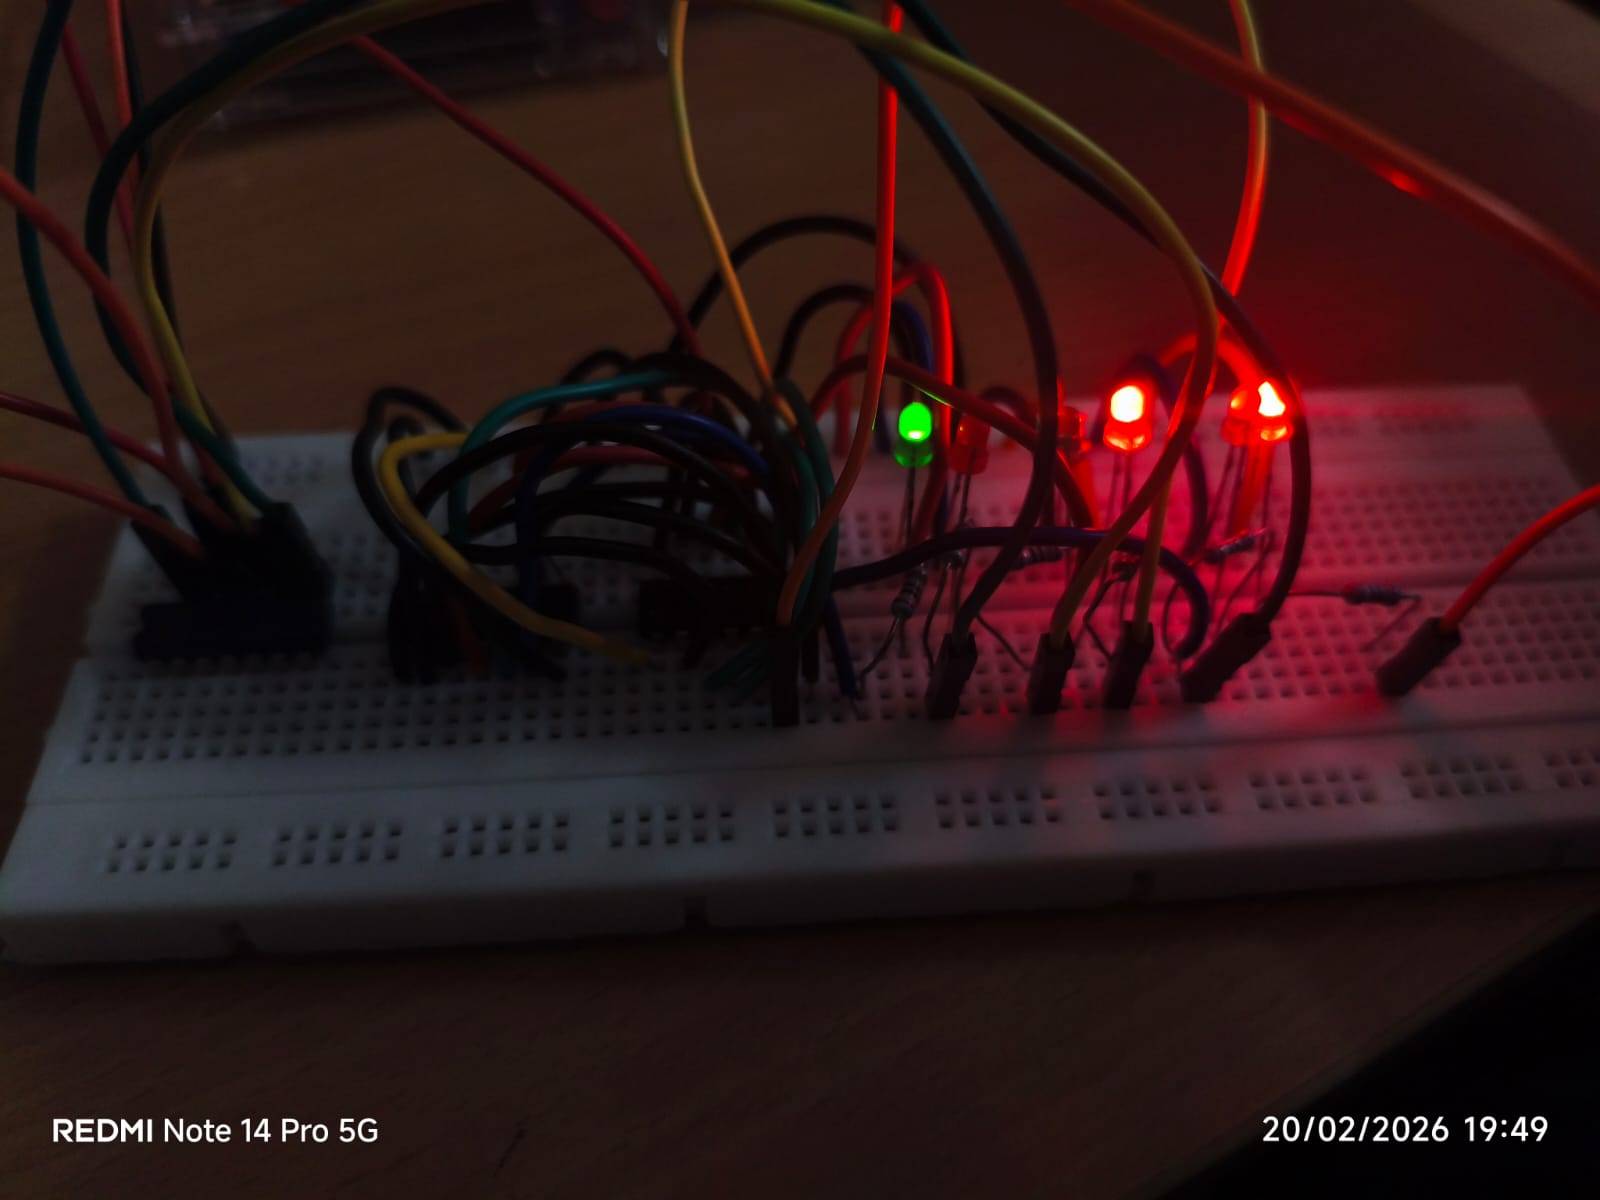
\includegraphics[width=0.5\columnwidth]{Figures/1st signal.jpeg}
\caption{LEDs blinking $ G_1R_2R_3$}
\label{fig:placeholder}
\end{figure}

\begin{figure}[H]
\centering
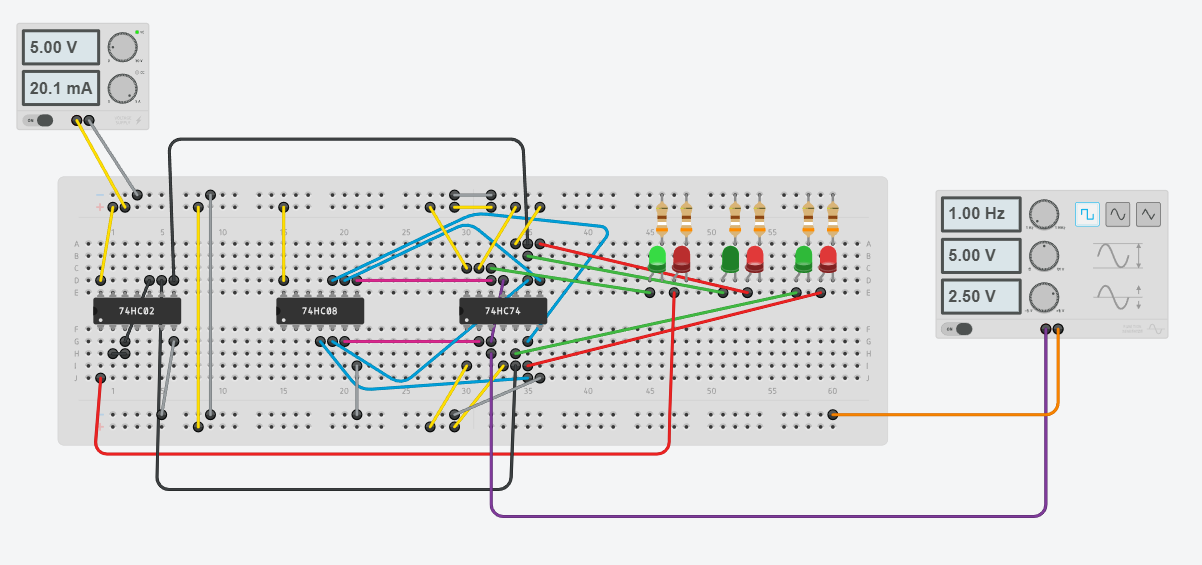
\includegraphics[width=0.8\columnwidth]{Figures/1st s.png}
\caption{LEDs blinking $ G_1R_2R_3$ (Simulation Result)}
\label{fig:placeholder}
\end{figure}

\begin{figure}[H]
\centering
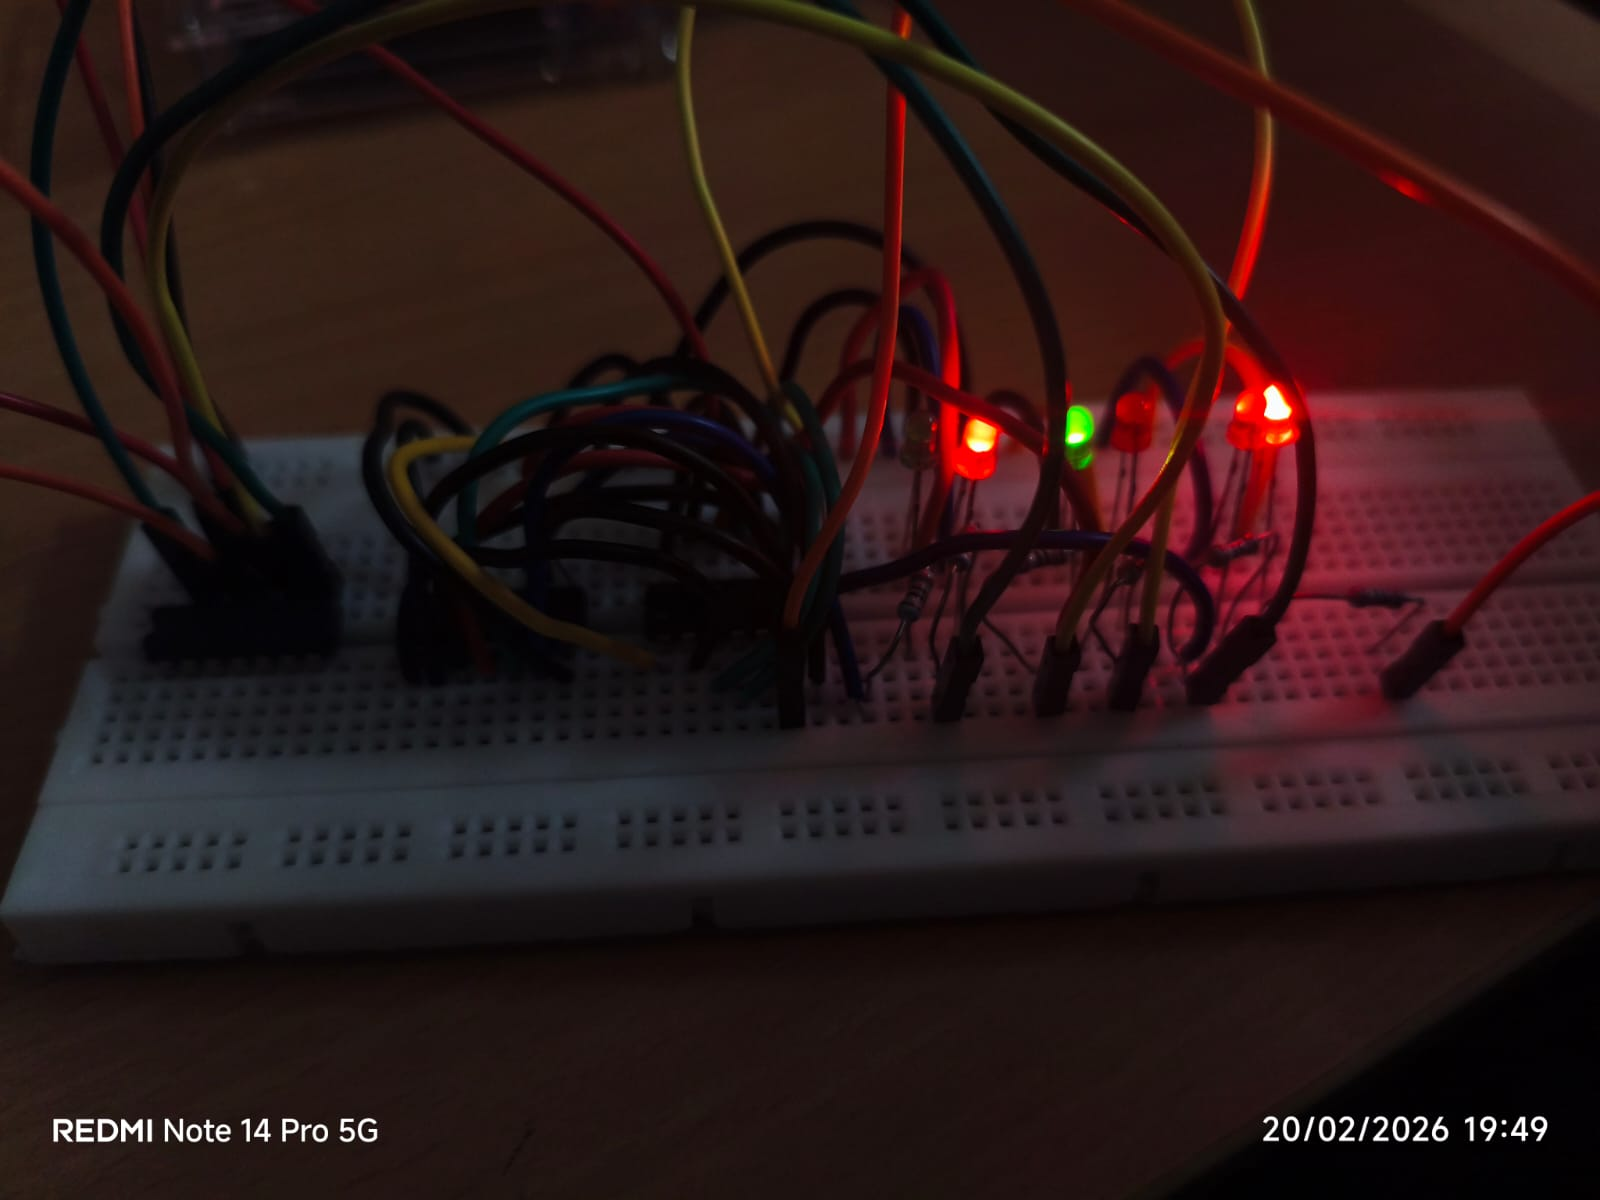
\includegraphics[width=0.5\columnwidth]{Figures/2nd signal.jpeg}
\caption{LEDs blinking $R_1G_2R_3$}
\label{fig:placeholder}
\end{figure}

\begin{figure}[H]
\centering
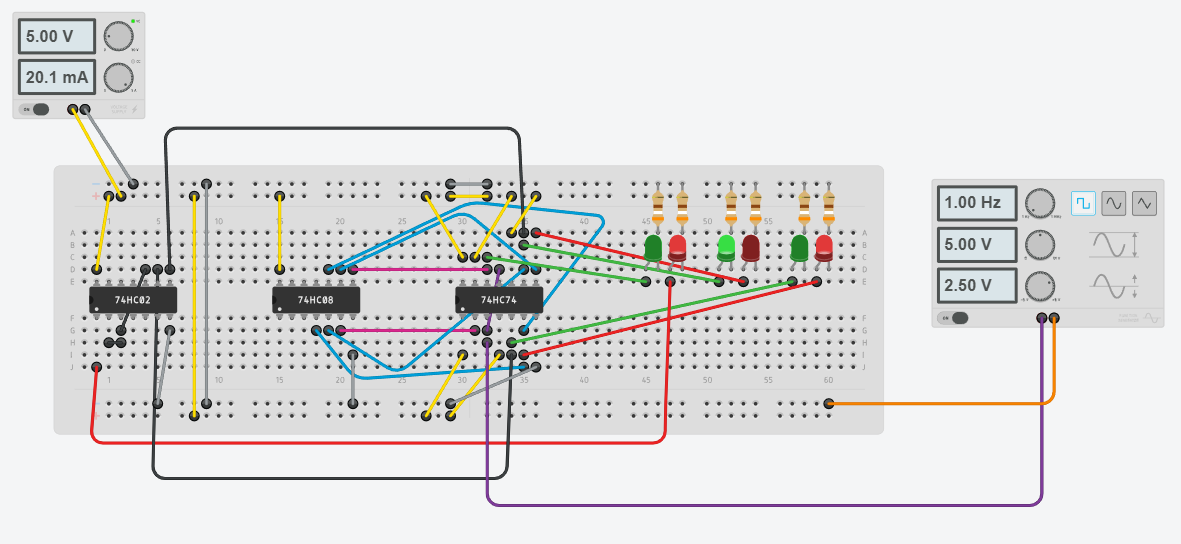
\includegraphics[width=0.8\columnwidth]{Figures/2nd s.png}
\caption{LEDs blinking $R_1G_2R_3$ (Simulation Result)}
\label{fig:placeholder}
\end{figure}

\begin{figure}[H]
\centering
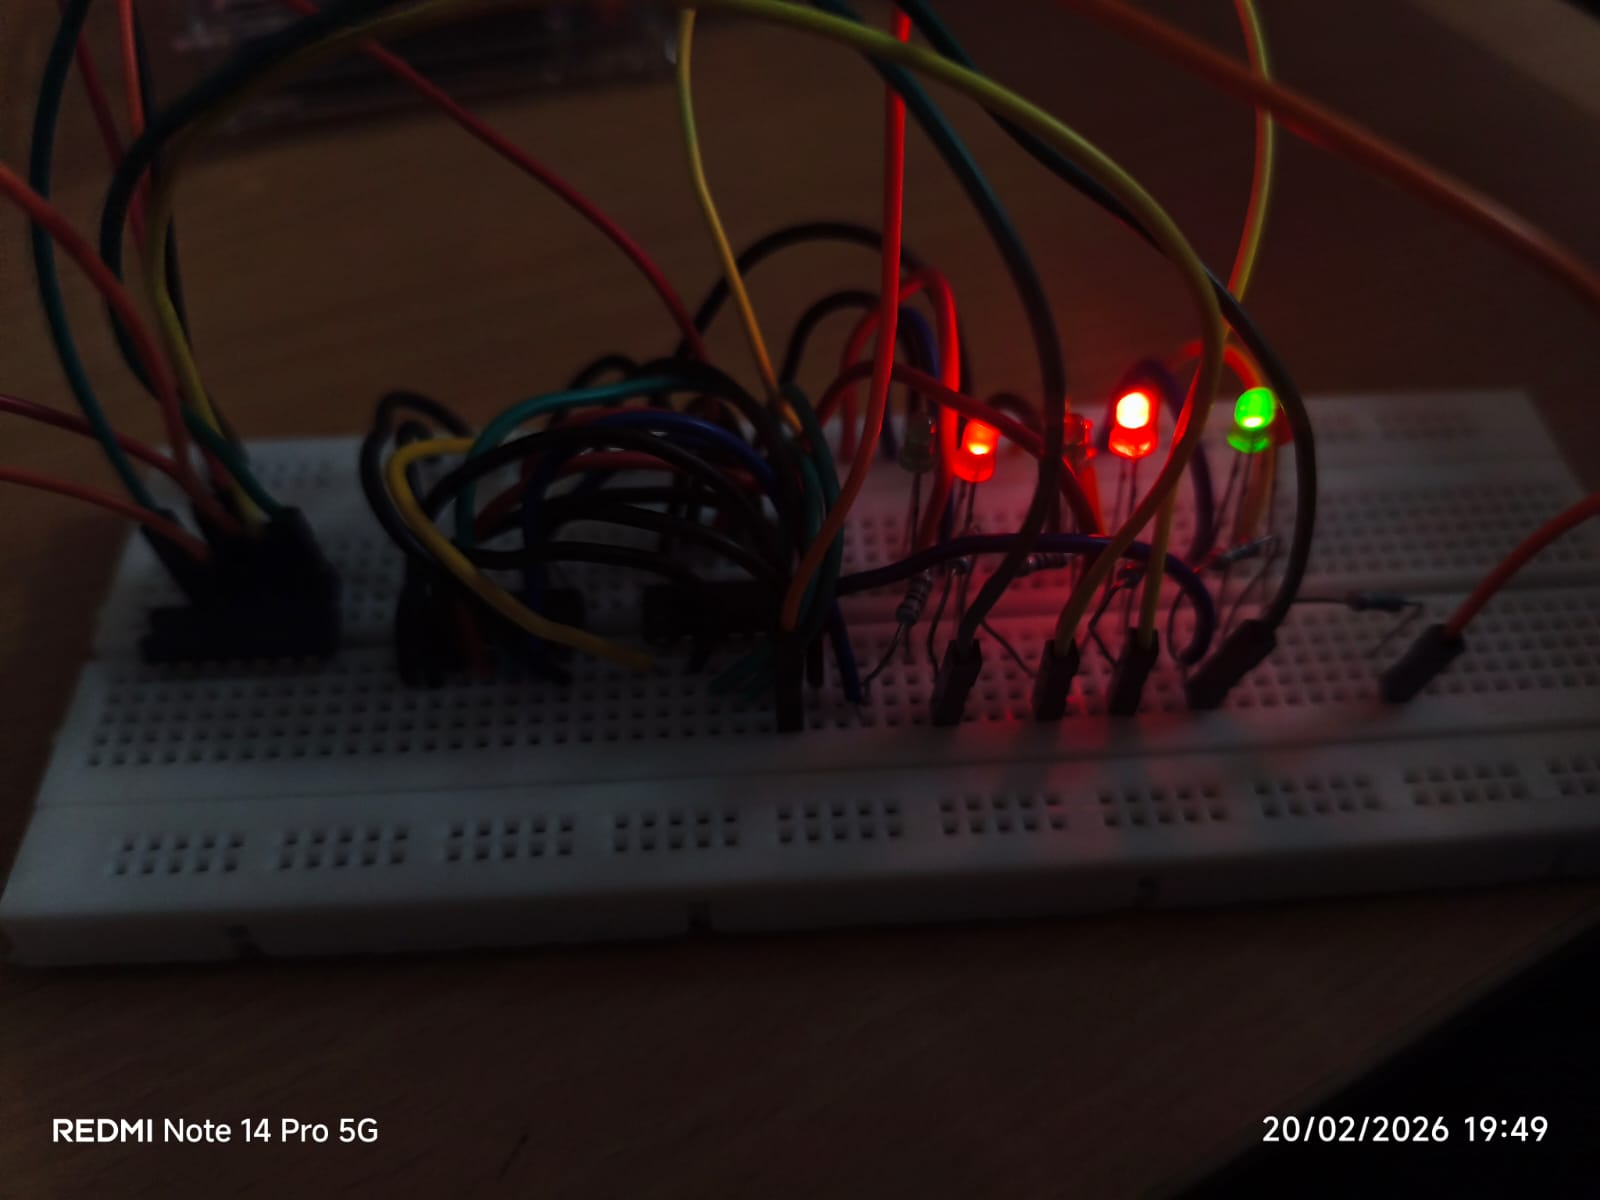
\includegraphics[width=0.5\columnwidth]{Figures/3rd signal.jpeg}
\caption{LEDs blinking $R_1R_2G_3 $}
\label{fig:placeholder}
\end{figure}

\begin{figure}[H]
\centering
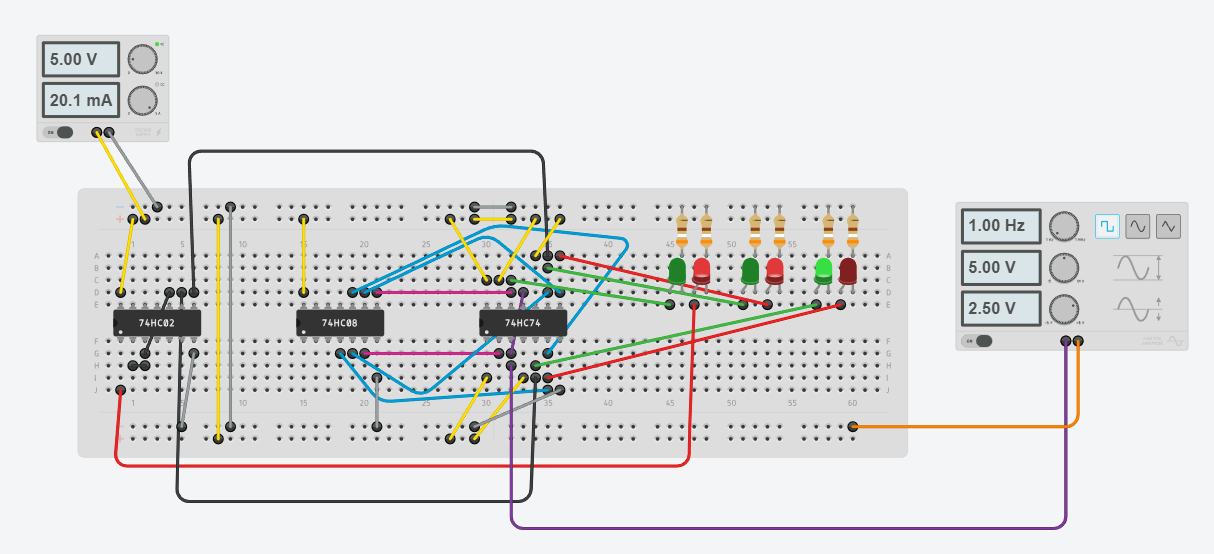
\includegraphics[width=0.8\columnwidth]{Figures/3rd s.png}
\caption{LEDs blinking $R_1R_2G_3$ (Simulation Result)}
\label{fig:placeholder}
\end{figure}

\textbf{Conclusion:}\\
The traffic light controller for a three-road junction was successfully designed and implemented using D flip-flops, logic gates, and an Arduino-generated clock signal. The state transition table was derived correctly, and the required Boolean expressions were implemented using combinational logic.\\

The experimental results matched the theoretical state transitions, thereby validating the correctness of the design.
\end{document}
